\documentclass[10pt, export]{beamer}

\usepackage[utf8]{inputenc}
\usepackage[T1]{fontenc}
    
\usepackage{standalone}
    
\usepackage[acronym]{glossaries}
    
\usepackage{enumitem}
    
\usepackage{xcolor}
    
\usepackage{multirow}
\usepackage{multicol}
    
\usepackage{array}
\newcolumntype{x}[1]{>{\centering\let\newline\\\arraybackslash\hspace{0pt}}p{#1}}
\usepackage{booktabs}
    
\usepackage{siunitx}
\usepackage{mathrsfs, amsmath}
    
\usepackage{graphicx}
\usepackage[font={small, color=IGNDarkGrey}, labelformat=empty]{caption}
\usepackage{subcaption}
\DeclareCaptionFont{tiny}{\tiny}
% \captionsetup[subtable]{labelfont={tiny, bf},textfont=normalfont,justification=raggedright}
\captionsetup[subfigure]{labelfont={tiny, bf},textfont=tiny,justification=raggedright}
\usepackage{adjustbox}

\usepackage{pifont}
\newcommand{\cmark}{{\color{green} \ding{51}}}%
\newcommand{\xmark}{{\color{red} \ding{55}}}%
    
\usepackage{hyperref}
    
\usepackage[
        mcite,
        backend=bibtex,
        style=verbose,
        citestyle=authoryear,
        bibstyle=numeric,
        sorting=none,
        autocite=footnote,
        maxnames=2,
        hyperref=true,
        natbib=true,
        abbreviate=true
    ]{biblatex}
\bibliography{references}
\setbeamerfont{footnote}{size=\tiny}


\usetheme{ign}


\newacronym{acr::lod}{LoD}{Level of Detail}
\newacronym{acr::elod}{eLoD}{evaluation Level of Detail}
\newacronym{acr::lidar}{LiDAR}{Light Detection and Ranging}
\newacronym{acr::dsm}{DSM}{Digital Surface Model}
\newacronym{acr::gui}{GUI}{Graphical User Interface}

\title{Semantic 3D building model evaluation}
\subtitle{}
\institute[LaSTIG STRUDEL]{Univ. Paris Est, LaSTIG STRUDEL, IGN, ENSG}
\date{\today}
\author[O.Ennafii]{Oussama Ennafii}


\begin{document}

    \begin{frame}[plain]
        \titlepage{}
    \end{frame}

    \section{Introduction}
        \begin{frame}{Context: 3D model vs. 3D mesh}
            \begin{itemize}[label=$\blacktriangleright$, font=\color{IGNGreen}, itemsep=2em]
                \item<1-> 3D urban model $\longleftrightarrow$ polyhedral surface representing a building.
                \item<2-> a 3D model facet $\longleftrightarrow$ an architectural feature.
            \end{itemize}
            \uncover<3>{
                \begin{figure}
                    \includestandalone[mode=buildnew, width=\textwidth]{lods}
                \end{figure}
            }
        \end{frame}
        \begin{frame}{Motivation}
            \only<1-4>{
                \begin{itemize}[label=$\blacktriangleright$, font=\color{IGNGreen}, itemsep=2em]
                    \item<1-> Automatic urban modeling: an active research area~\citep{Musialski2012};
                    \item<2-> Results seamless but lack generality and often erroneous~\citep{rottensteiner2014results};
                    \begin{itemize}[label=$\longrightarrow$]
                        \item<3-> labourious manual corrections.
                    \end{itemize}
                    \item<4-> Urban 3D model semantic diagnostic \textcolor{purple}{not well studied}~\citep{nguatem2017modeling};
                \end{itemize}
            }
            \only<5->{
                \begin{itemize}[label=Goal $\longrightarrow$, font=\color{purple}, leftmargin=2cm]
                    \item<5-> Detect and describe semantic errors that affect building 3D models.
                \end{itemize}
                \begin{itemize}[label=$\blacktriangleright$, font=\color{IGNGreen}, itemsep=2em]
                    \item<6-> Semantic errors independent from \textbf{reconstruction methods} and \textbf{urban scenes}.
                    \item<7-> \textbf{Transferability}, and hence scallability, of the evaluation method.
                \end{itemize}
            }
        \end{frame}
        \begin{frame}{Potential use}
            \begin{itemize}[label=$\blacktriangleright$, font=\color{IGNGreen}, itemsep=2em]
                \item<1-> Change detection;
                \item<2-> Urban models correction;
                \item<3-> Urban reconstruction method evaluation;
                \item<4-> Crowd reconstruction quality assessment.
            \end{itemize}
        \end{frame}

    \section{Methodology}
        \begin{frame}{Main ideas behind our approach}
            \begin{itemize}[label=$\blacktriangleright$, font=\color{IGNGreen}, itemsep=2em]
                \item<1-> Compile errors that affect building models in a taxonomy;
                \item<2-> Evaluation at building level $\Longrightarrow$ formulated as a supervised classification problem;
                \item<3-> Study in a \textbf{2.5D overhead (aerial)} modeling setting.
            \end{itemize}
        \end{frame}
        \begin{frame}{Taxonomy structure}
            Two criteria determine the taxonomy structure:
            \begin{itemize}[label=$\blacktriangleright$, font=\color{IGNGreen}, itemsep=2em]
                \item<2-> the \textbf{\acrfull{acr::lod}};
                \item<3-> the \textbf{\emph{finesse}}: the semantic evaluation level.
            \end{itemize}
            ~\\
            \uncover<4->{
                \begin{block}{Definition}
                    An error is of maximal \emph{finesse} $\Leftrightarrow$ it corresponds, semantically, to a unitary action required to correct the model. The error is called \emph{atomic}.
                \end{block}
            }
        \end{frame}
        \begin{frame}{Error taxonomy (\textit{finesse} $= 0$)}
            \begin{figure}
                \includestandalone[mode=buildnew, height=.7\textheight]{finesse_0_taxonomy}
            \end{figure}
        \end{frame}
        \begin{frame}{Error taxonomy (\textit{finesse} $= 1$)}
            \begin{figure}
                \includestandalone[mode=buildnew, height=.7\textheight]{finesse_1_taxonomy}
            \end{figure}
        \end{frame}
        \begin{frame}{Error taxonomy (\textit{finesse} $= 2$)}
            \begin{figure}
                \includestandalone[mode=buildnew, height=.7\textheight]{finesse_2_taxonomy}
            \end{figure}
        \end{frame}
        \begin{frame}{Error taxonomy (\textit{finesse} $= 2$)}
            \begin{figure}
                \includestandalone[mode=buildnew, height=.7\textheight]{finesse_2_taxonomy_lods}
            \end{figure}
        \end{frame}
        \begin{frame}{Error taxonomy (\textit{finesse} $= 3$)}
            \begin{figure}
                \includestandalone[mode=buildnew, width=\textwidth]{finesse_3_bul_taxonomy}
            \end{figure}
        \end{frame}
        \begin{frame}{Building \textit{atomic} errors: 2.5D overhead reconstruction case}
            \begin{figure}
                \begin{center}
                    \begin{subfigure}{.28\textwidth}
                        \fbox{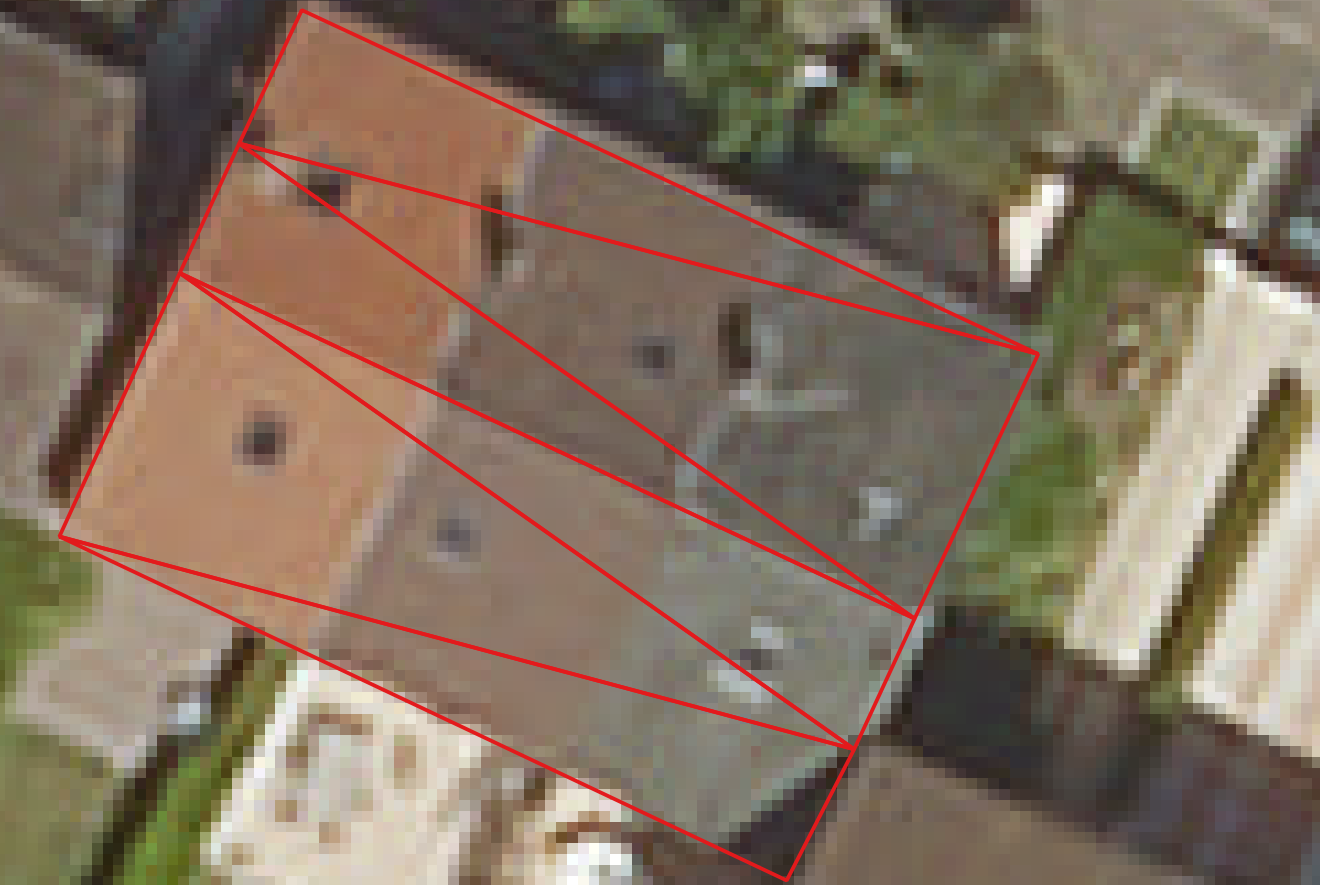
\includegraphics[width=\textwidth]{images/errors/building/under_segmentation}}
                        \caption{\label{fig::bul_under} Under segmentation}
                    \end{subfigure}
                    \hspace{10pt}
                    \begin{subfigure}{.28\textwidth}
                        \fbox{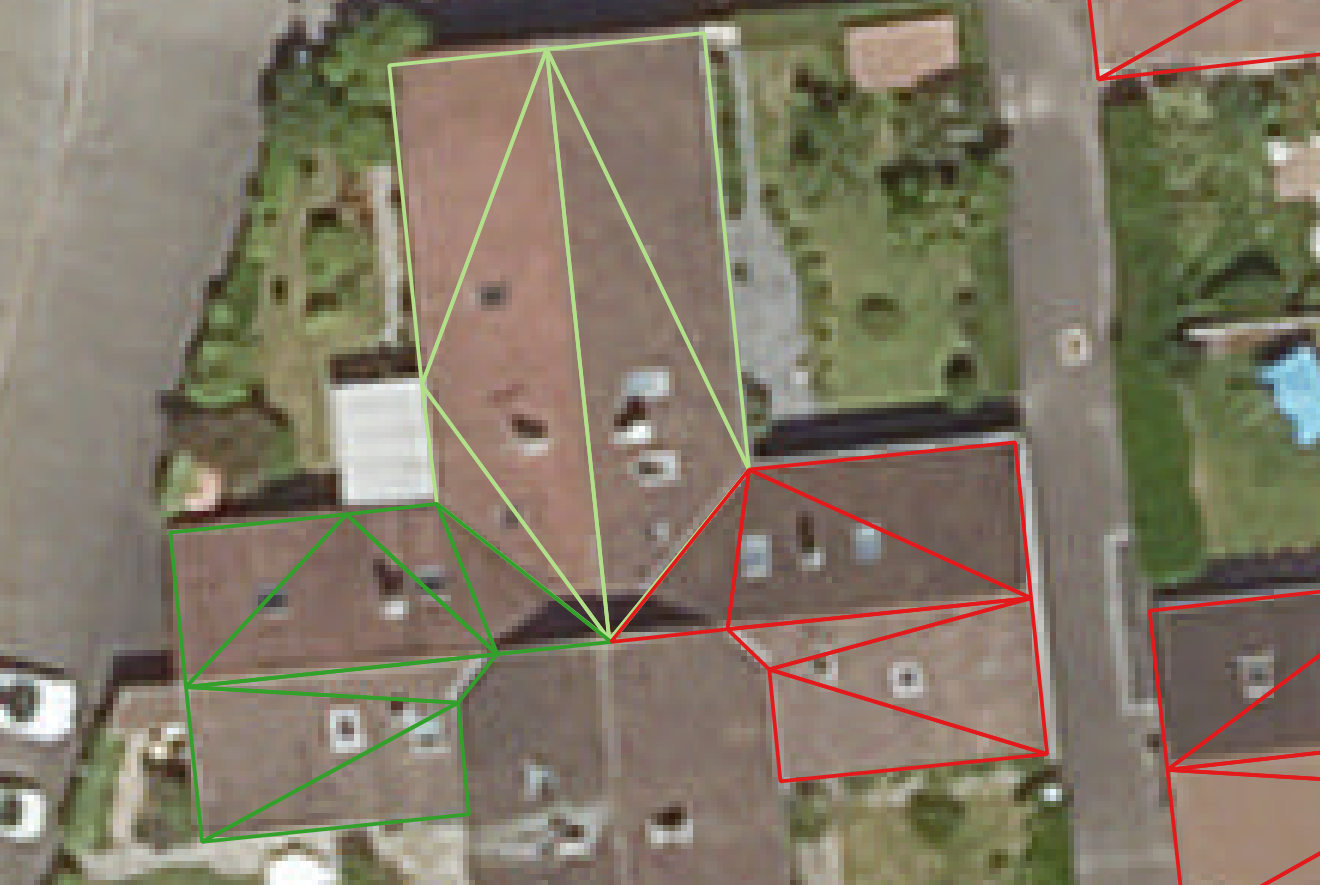
\includegraphics[width=\textwidth]{images/errors/building/over_segmentation}}
                        \caption{\label{fig::bul_over} Over segmentation}
                    \end{subfigure}
                    \hspace{10pt}
                    \begin{subfigure}{.28\textwidth}
                        \fbox{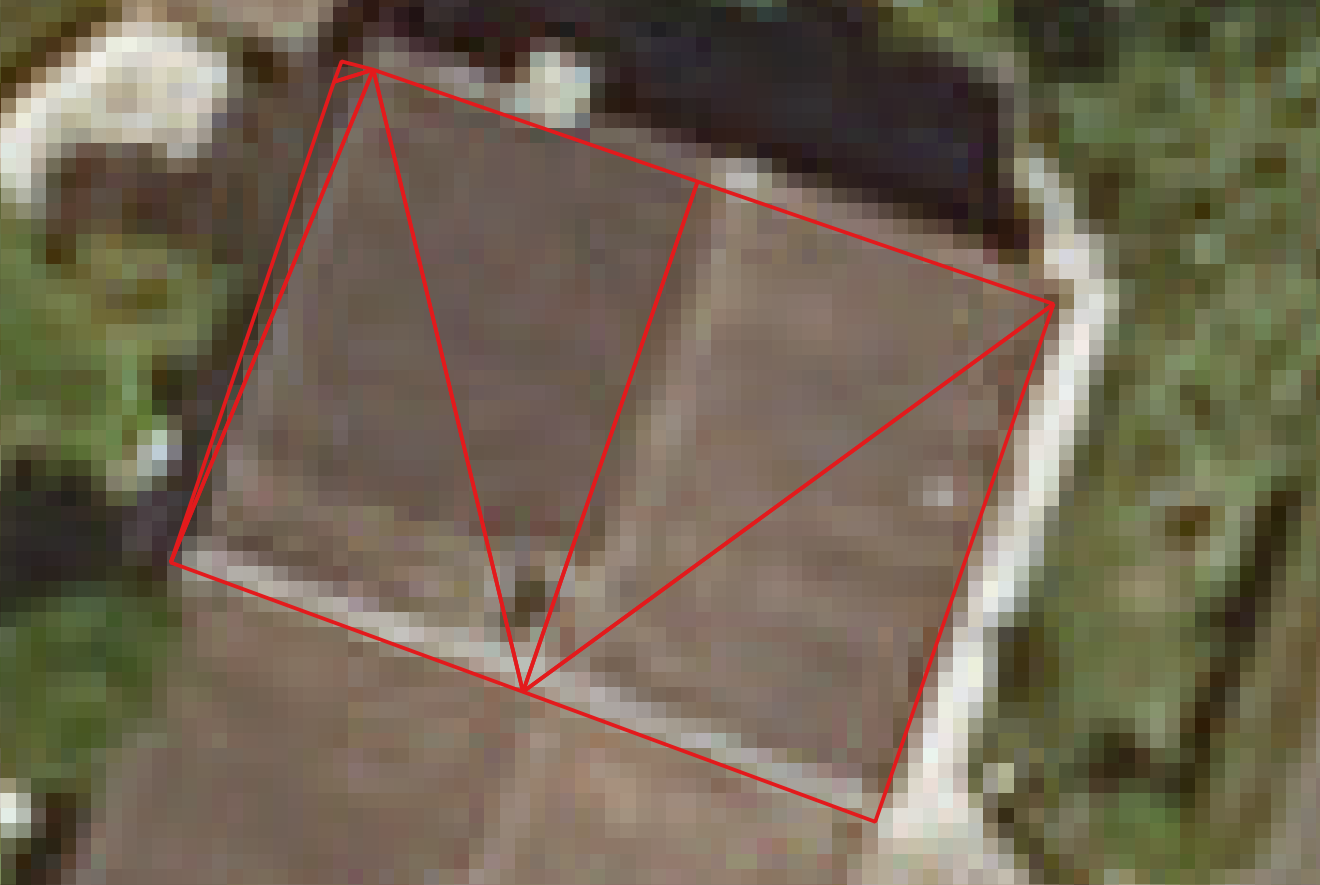
\includegraphics[width=\textwidth]{images/errors/building/footprint}}
                        \caption{\label{fig::bul_footprint} Imprecise border}
                    \end{subfigure}
                    \hspace{10pt}
                    \begin{subfigure}{.28\textwidth}
                        \fbox{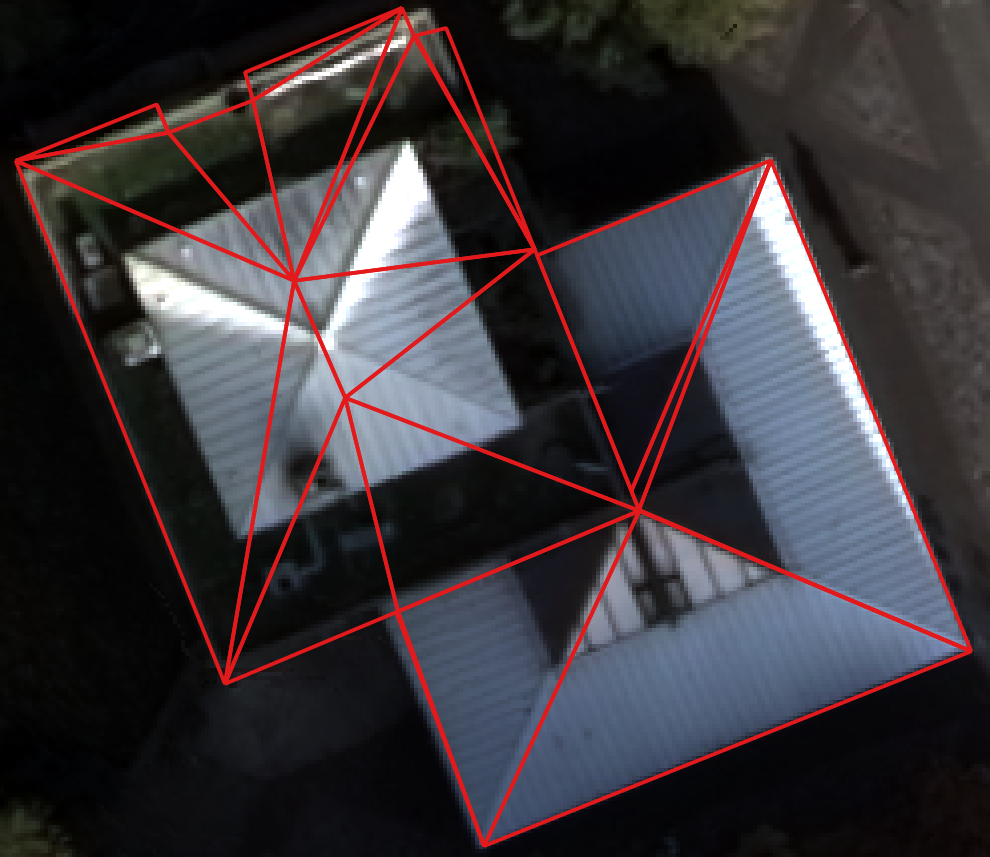
\includegraphics[width=\textwidth]{images/errors/building/footprint_topology}}
                        \caption{\label{fig::bul_height} Inaccurate topology}
                    \end{subfigure}
                \end{center}
            \end{figure}
        \end{frame}
        \begin{frame}{Error taxonomy (\textit{finesse} $= 3$)}
            \begin{figure}
                \includestandalone[mode=buildnew, width=\textwidth]{finesse_3_all_taxonomy}
            \end{figure}
        \end{frame}
        \begin{frame}{Facet \textit{atomic} errors: 2.5D overhead reconstruction case}
            \begin{figure}
                \begin{center}
                    \begin{subfigure}{.28\textwidth}
                        \fbox{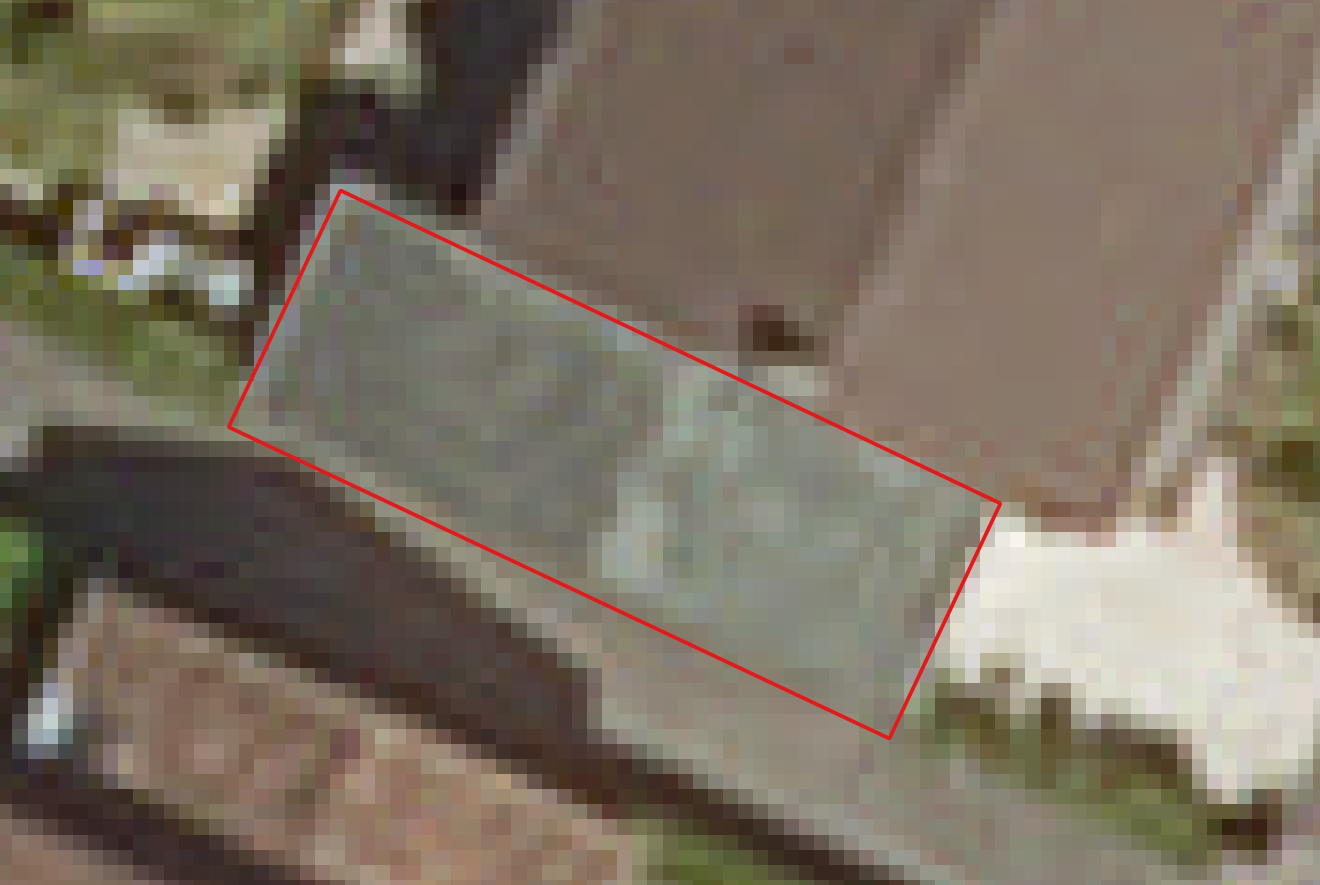
\includegraphics[width=\textwidth]{images/errors/facet/under_segmentation}}
                        \caption{\label{fig::fac_under} Under segmentation}
                    \end{subfigure}
                    \hspace{10pt}
                    \begin{subfigure}{.28\textwidth}
                        \fbox{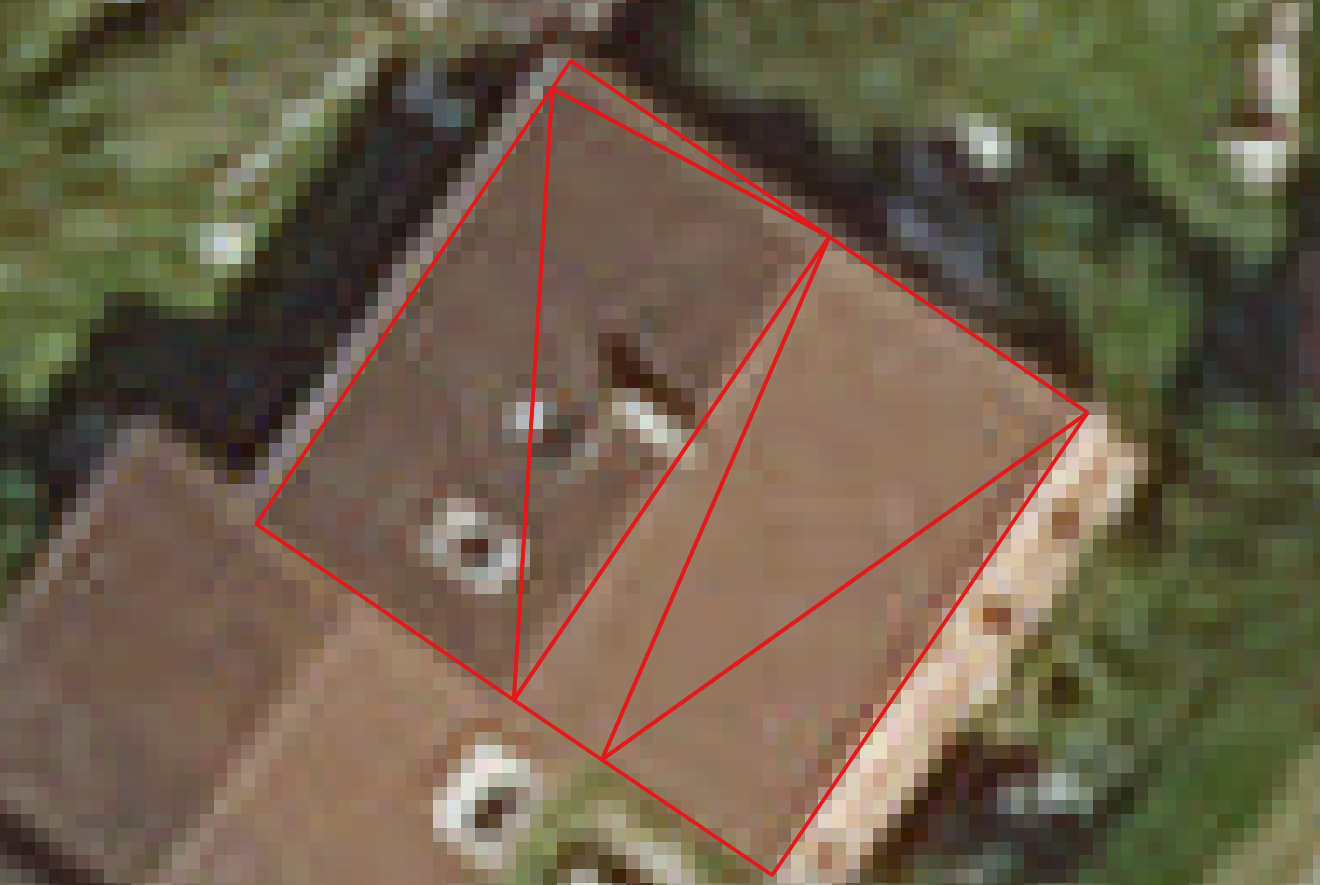
\includegraphics[width=\textwidth]{images/errors/facet/over_segmentation}}
                        \caption{\label{fig::fac_over} Over segmentation}
                    \end{subfigure}
                    \hspace{10pt}
                    \begin{subfigure}{.28\textwidth}
                        \fbox{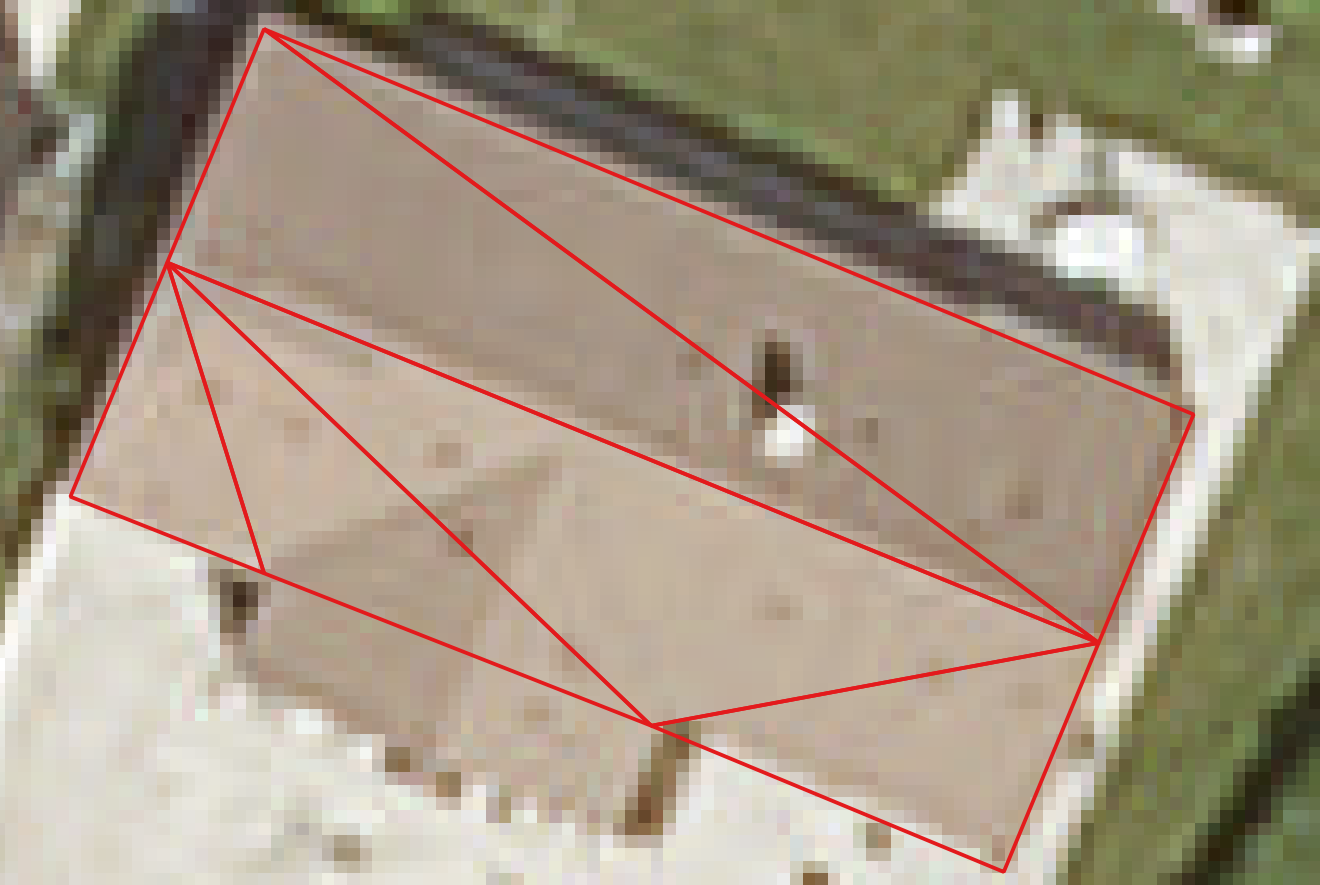
\includegraphics[width=\textwidth]{images/errors/facet/mis_segmentation}}
                        \caption{\label{fig::fac_footprint} Imprecise borders}
                    \end{subfigure}
                    \hspace{10pt}
                    \begin{subfigure}{.28\textwidth}
                        \fbox{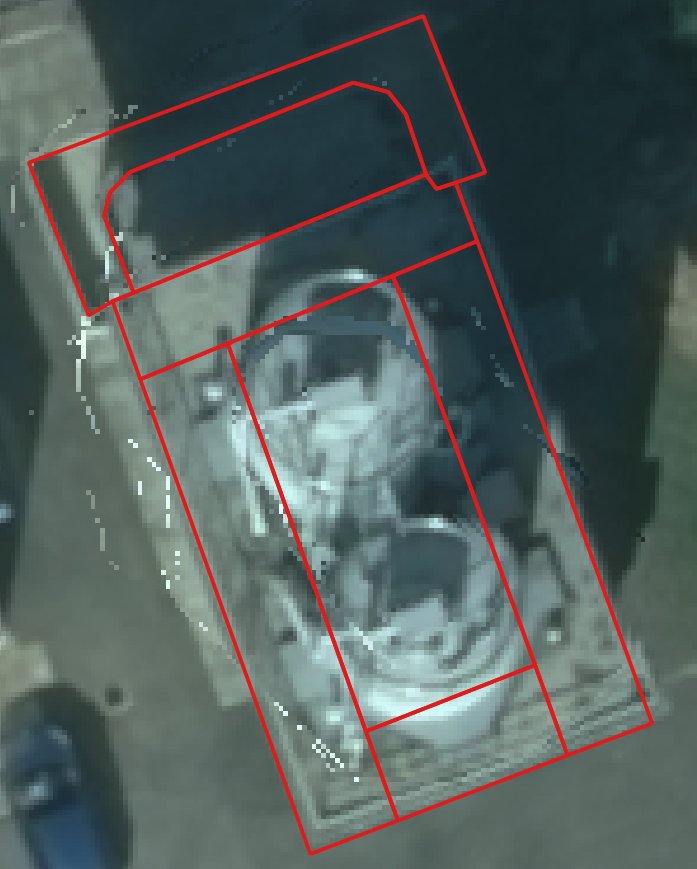
\includegraphics[width=\textwidth]{images/errors/facet/topology}}
                        \caption{\label{fig::fac_height} Inaccurate topology}
                    \end{subfigure}
                    \hspace{10pt}
                    \begin{subfigure}{.28\textwidth}
                        \fbox{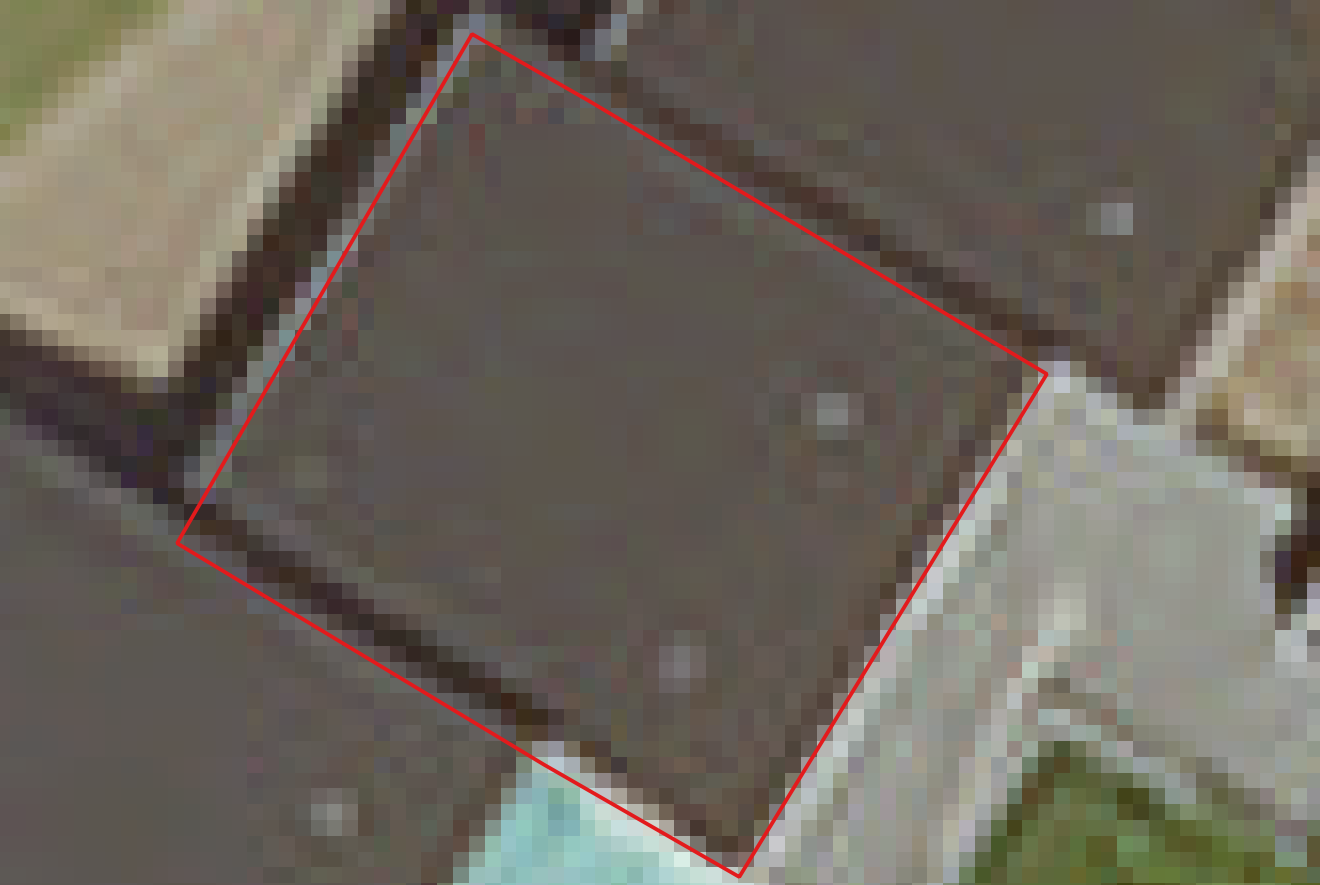
\includegraphics[width=\textwidth]{images/errors/facet/slope}}
                        \caption{\label{fig::fac_height} Imprecise geometry}
                    \end{subfigure}
                \end{center}
            \end{figure}
        \end{frame}

        \begin{frame}{The evaluation pipeline sketch}
            \begin{figure}
                \includegraphics[width=\textwidth]{graphical_abstract}
            \end{figure}
        \end{frame}
        \begin{frame}{Geometric features}
            \begin{figure}
                \includegraphics[height=.75\textheight]{geometric_features}
            \end{figure}
        \end{frame}
        \begin{frame}{Height-based features}
            \begin{figure}
                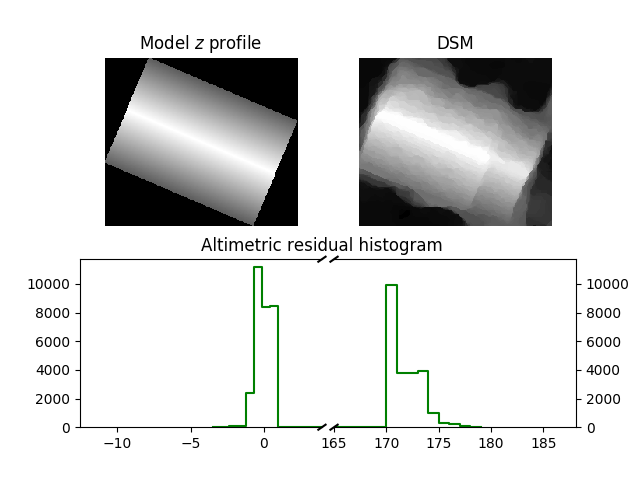
\includegraphics[height=.7\textheight]{images/altimetric_features}
            \end{figure}
        \end{frame}
        \begin{frame}{Image-based features}
            \begin{figure}
                \begin{subfigure}{.48\textwidth}
                    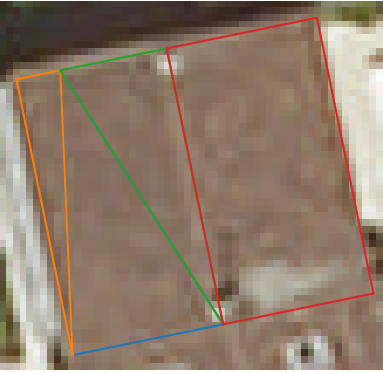
\includegraphics[width=\textwidth]{images/radio_vector}
                    \caption{\label{fig::ortho_sup} A building projection and the corresponding orthoimage.}
                \end{subfigure}
                \begin{subfigure}{.48\textwidth}
                    \includestandalone[mode=buildnew, width=\textwidth]{radiometric_features}
                    \caption{\label{fig::hist} For each facet edge, the cosine similarity is computed between its normal and the image gradient, on each intersecting pixel (in green).}
                \end{subfigure}
            \end{figure}
        \end{frame}

    \section{Experiments}
        \begin{frame}{Results using all features}
            \begin{table}
                \begin{center}
                    \scriptsize
                    \begin{tabular}{c c c c}
                        \toprule
                        & Elancourt & Nantes & Paris 13 \\
                        \midrule
                        \# samples & 2009 & 748 & 478 \\
                        \bottomrule
                    \end{tabular}
                    \caption{\scriptsize Dataset statistics}
                    \uncover<2->{
                        \begin{tabular}{|x{1cm} | x{1.3cm} x{1.3cm} | x{1.2cm} x{1.2cm} | x{1.2cm} x{1.2cm}|}
                            \hline
                            & \multicolumn{2}{x{3cm}|}{\textbf{Elancourt (10-cross val.)}} & \multicolumn{2}{x{2.4cm}|}{\textbf{Elancourt $\rightarrow$ Nantes}} & \multicolumn{2}{x{2.5cm}|}{\textbf{Elancourt $\rightarrow$ Paris 13}}\\
                            \cline{2-7}
                            &\textbf{Recall} & \textbf{Prec.} & \textbf{Recall} & \textbf{Prec.} & \textbf{Recall} & \textbf{Prec.} \\
                            \hline
                            \textit{BOS} & 90.83 & 76.14 & \textcolor{IGNDarkGreen}{93.12} & \textcolor{red}{42.61} & \textcolor{IGNDarkGreen}{96.53} & \textcolor{red}{43.82} \\
                            \hline
                            \textit{BUS} & 39.32 & 71.81 & \textcolor{red}{8.82} & 66.67 & \textcolor{red}{0} & \textcolor{red}{---} \\
                            \hline
                            \textit{BImB} & 16.75 & 68.0 & \textcolor{red}{2.02} & 33.33 & \textcolor{red}{0} & \textcolor{red}{---} \\
                            \hline
                            \textit{BInT} & 11.11 & 91.67 & 0.88 & 100 & 3.95 & 50.0 \\
                            \hline
                            \hline
                            \textit{FOS} & 98.91 & 98.84 & \textcolor{IGNDarkGreen}{98.33} & \textcolor{IGNDarkGreen}{97.92} & \textcolor{IGNDarkGreen}{97.19} & \textcolor{IGNDarkGreen}{97.58} \\
                            \hline
                            \textit{FUS} & 1.27 & 66.67 & \textcolor{IGNDarkGreen}{13.81} & \textcolor{IGNDarkGreen}{63.04} & 8.36 & 95.83 \\
                            \hline
                            \textit{FImB} & 7.42 & 100 & \textcolor{IGNDarkGreen}{46.34} & 65.52 & 11.80 & 60.71 \\
                            \hline
                            \textit{FImT} & 3.33 & 100 & 9.09 & 100 & 0 & 0 \\
                            \hline
                            \textit{FIG} & 79.02 & 71.82 & \textcolor{IGNDarkGreen}{94.17} & 70.70 & \textcolor{IGNDarkGreen}{86.16} & \textcolor{IGNDarkGreen}{88.47} \\
                            \hline
                        \end{tabular}
                        \caption{\scriptsize Test results using \textbf{Random Forest} ($max\ depth = 4$ \& $\# trees = 1000$) trained on Elancourt.}
                    }
                \end{center}
            \end{table}
        \end{frame}
        \begin{frame}{Some failure cases on Elancourt}
            \begin{figure}
                \begin{center}
                \tiny
                    \begin{tabular}{| x{.06\textwidth} | x{.035\textwidth} | x{.035\textwidth} || x{.06\textwidth} | x{.035\textwidth} | x{.035\textwidth} || x{.06\textwidth} | x{.035\textwidth} | x{.035\textwidth} || x{.06\textwidth} | x{.035\textwidth} | x{.035\textwidth} |}
                        \hline
                        \multicolumn{3}{| c ||}{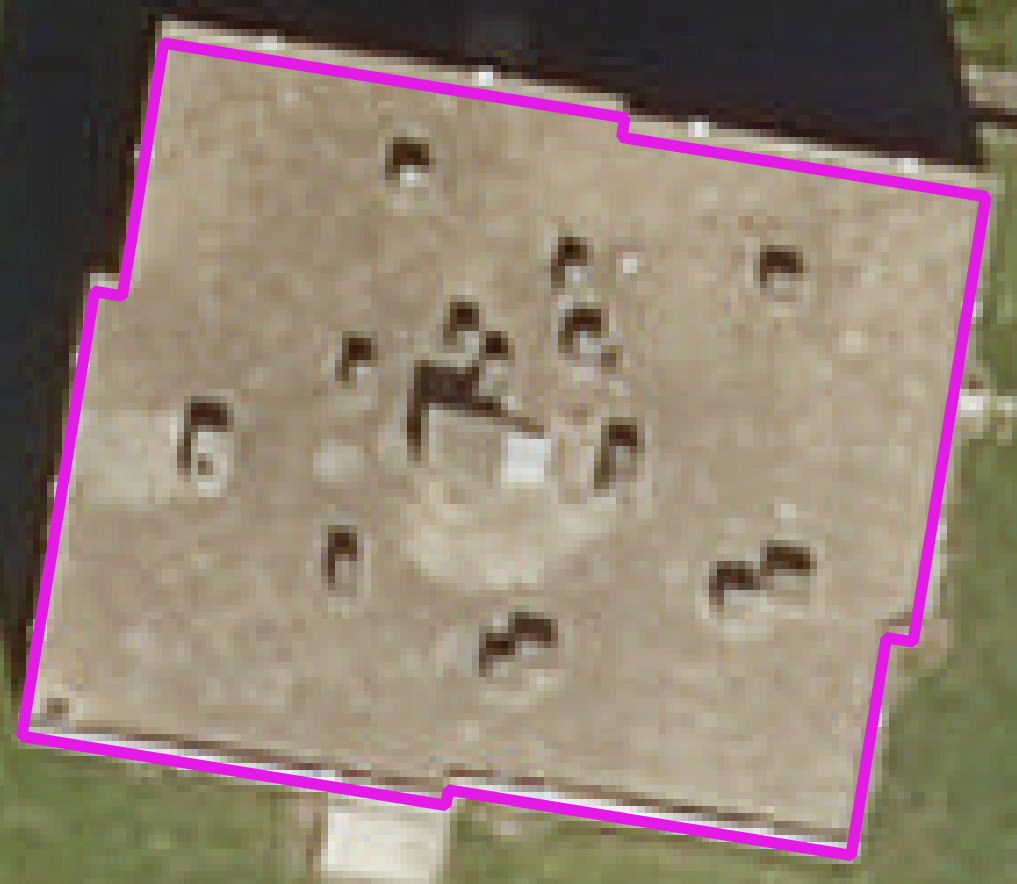
\includegraphics[width=.2\textwidth,valign=m,margin=1pt 1pt]{images/prediction_results/valid_as_bul_over}} & \multicolumn{3}{ c ||}{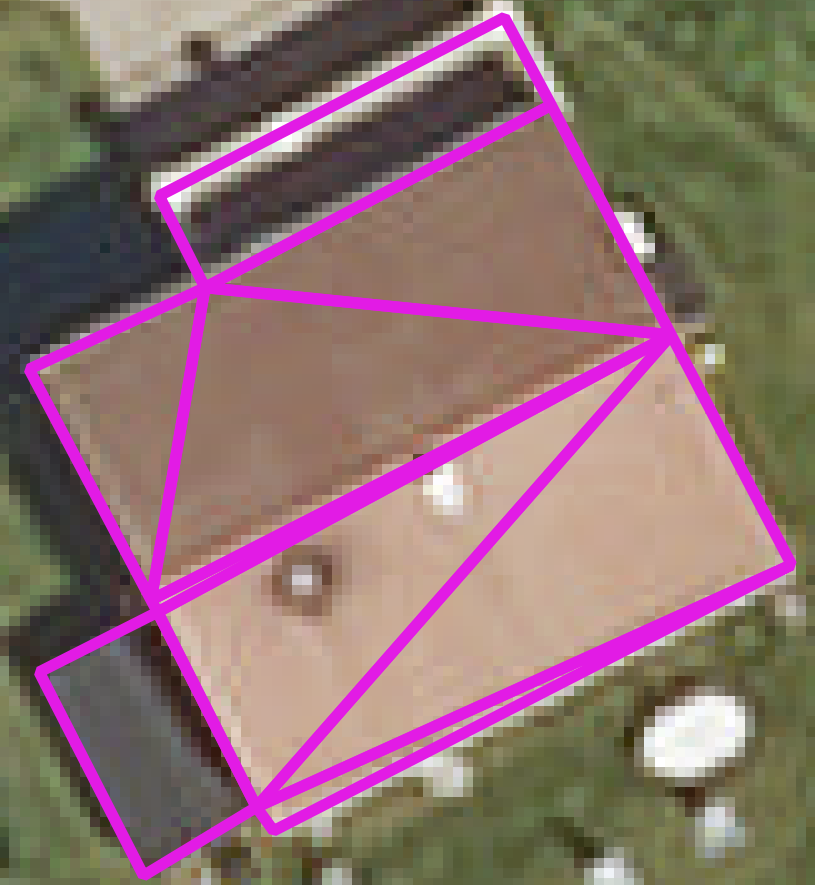
\includegraphics[width=.2\textwidth,valign=m,margin=0cm 1pt]{images/prediction_results/no_imprec_no_fac_over}} & \multicolumn{3}{ c ||}{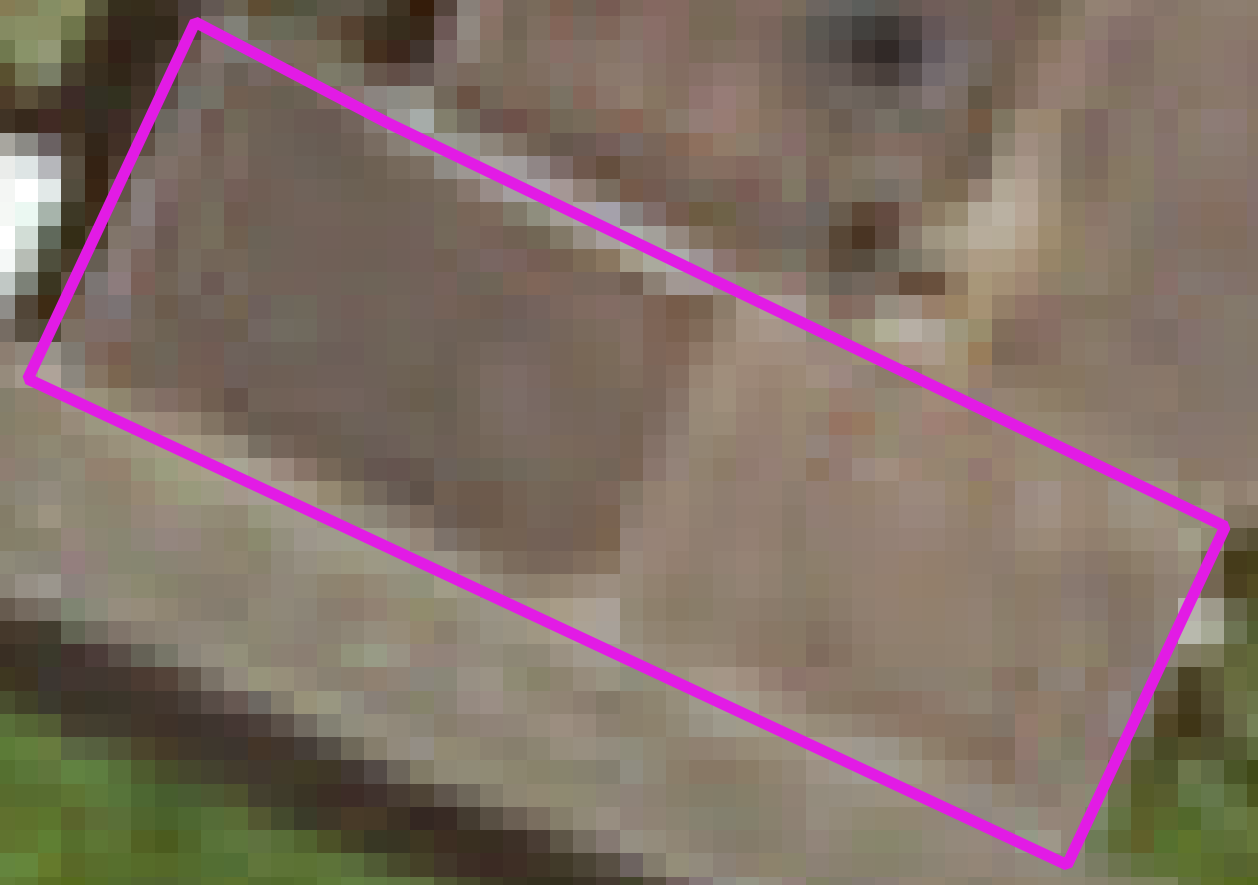
\includegraphics[width=.2\textwidth,valign=m,margin=0cm 1pt]{images/prediction_results/no_under_seg}} & \multicolumn{3}{ c |}{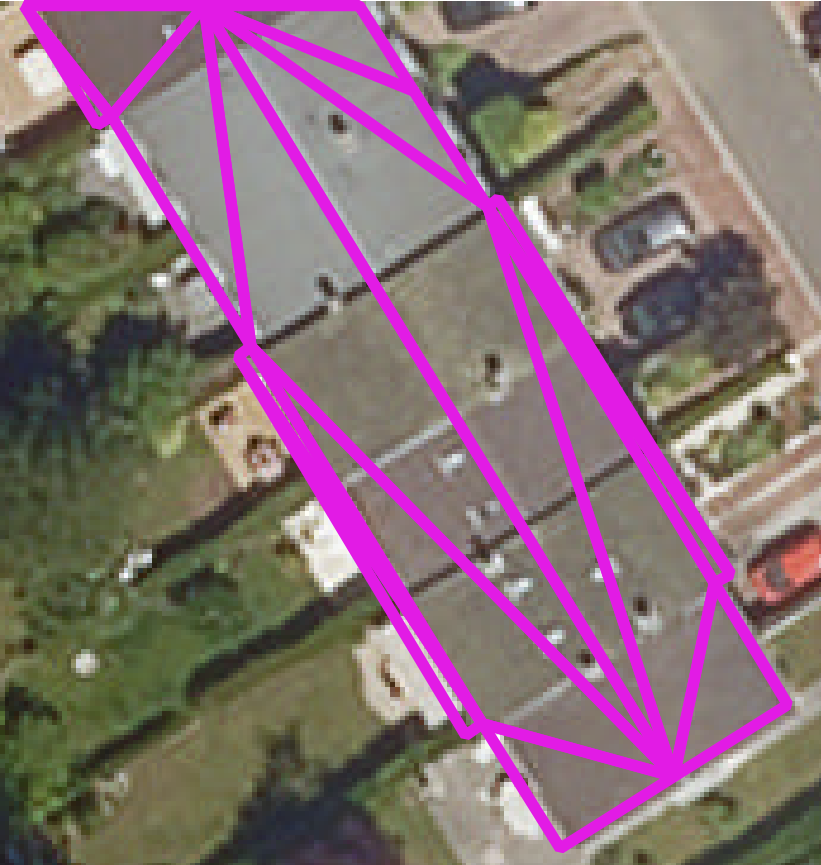
\includegraphics[width=.2\textwidth,valign=m,margin=0cm 1pt]{images/prediction_results/no_bul_under_seg}} \\
                        \hline
                        \textbf{Errors} & \textbf{G.T.} & \textbf{Pred.} & \textbf{Errors} & \textbf{G.T.} & \textbf{Pred.} & \textbf{Errors} & \textbf{G.T.} & \textbf{Pred.} & \textbf{Errors} & \textbf{G.T.} & \textbf{Pred.}\\
                        \hline
                        \textit{BOS} & \xmark & \cmark & \textit{BUS} & \xmark & \cmark & \textit{BOS} & \cmark & \cmark & \textit{BOS} & \cmark & \xmark \\
                        Valid & \cmark & \xmark & \textit{FIG} & \cmark & \xmark & \textit{FUS} & \cmark & \xmark &  \textit{FOS} & \cmark & \xmark \\
                            &  &  & \textit{FOS} & \cmark & \xmark &  &  &  & \textit{BUS} & \cmark & \xmark \\
                            &  &  &  &  &  &  &  &  &  \textit{BImB} & \cmark & \cmark \\
                        \hline
                    \end{tabular}
                \end{center}
            \end{figure}
        \end{frame}
    
    \section{Conclusion}
        \begin{frame}{\textcolor{yellow}{Conclusion} \& \textcolor{purple}{Perspectives}}
            \begin{itemize}[label=$\blacktriangleright$, font=\color{yellow}, itemsep=2em]
                \item \textbf{Flexible, robust and hierarchical} taxonomy;
                \item \textbf{Fast, lightweight and modular} pipeline for model evaluation;
                \item Baseline for geometric, image-based and height-based features;
            \end{itemize}
            \uncover<2->{
                ~\\
                Future work:
                \begin{itemize}[label=$\blacktriangleright$, font=\color{purple}, itemsep=2em]
                    \item Dataset augmentation $\longrightarrow$ \textbf{Simulate errors} from the taxonomy based on reference data;
                    \item Extend to richer features $\longrightarrow$ Graph kernels, deep learning.
                \end{itemize}
            }
        \end{frame}
\end{document}